\chapter{Gesamtsystem}
% ================ Einstellungen =======================
\thispagestyle{fancy} \rhead{\slshape Gesamtsystem}
% ======================================================

Abbildung XYZ zeigt das grobe Gesamtsystem des Dojos. Die einzelnen Abschnitte dieses Berichts orientieren sich nach den Blöcken und deren Funktion im Gesamtsystem. In Abschnitt \textbf{\ref{Software} \nameref{Software}} wird die Computersoftware erklärt, welche verwendet wird um den Dojo zu konfigurieren. Der Abschnitt \textbf{\ref{Energieversorgung} \nameref{Energieversorgung}} befasst sich mit dem Akku, der Lade -schaltung und überwachnug, sowie der Spannungsversorgung. Im Abschnitt \textbf{\ref{USB} \nameref{USB}} wird erläutert, wie über die USB-Schnittstelle mit dem Mikrocontroller kommuniziert wird und wie Audiofiles auf die SD-Karte übertragen werden. Der Abschnitt \textbf{\ref{Audioausgabe} \nameref{Audioausgabe}} behandelt die Verarbeitung und Ausgabe der Audiofiles. Der nächste Abschnitt \textbf{\ref{Bluetooth} \nameref{Bluetooth}} befasst sich mit dem Bluetooth. Das heisst, mit den Beacons zur Erkennung der Kunstobjekte und dem Bluetoothmodul im Dojo für den Empfang. Wie die Firmware als Gesamtsystem funktioniert, erfährt man im Abschnitt \textbf{\ref{Firmware} \nameref{Firmware}} detailliert.

\begin{figure}[h]
	\centering
	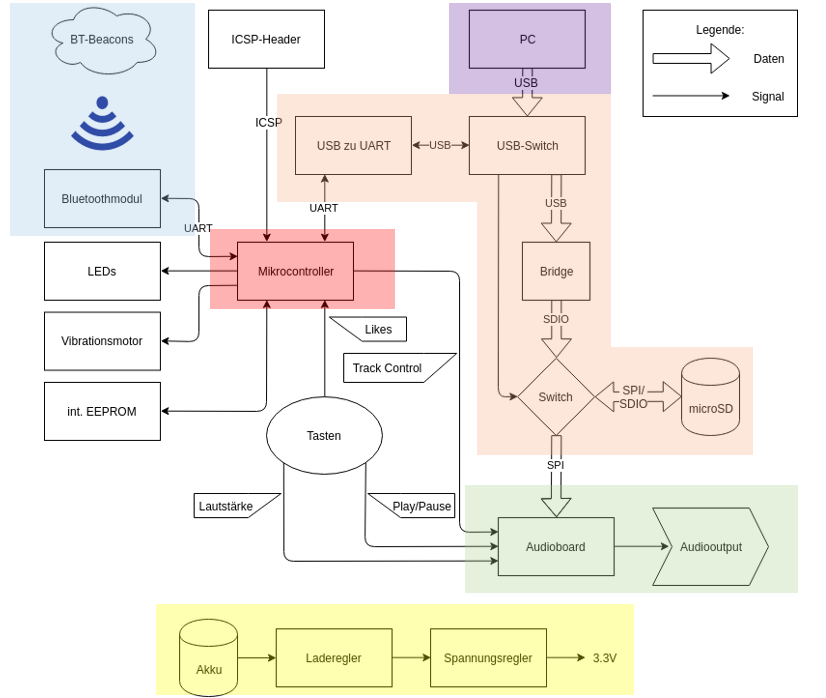
\includegraphics[width=\textwidth]{Bilder/Gesamtsystem.png}
	\caption{Blockschaltbild Gesamtsystem}
	\label{Blockschaltbild_Gesamtsystem}
\end{figure}
